\documentclass[a4paper,12pt,twoside]{scrreprt}
% Autor der Vorlage: Klaus Rheinberger, FH Vorarlberg
% 2017-02-20

%% Hilfe: z.B.
% empfohlener Einstieg: http://latex.tugraz.at/
% https://de.wikibooks.org/wiki/LaTeX-Kompendium:_Schnellkurs:_Erste_Schritte
% https://de.wikibooks.org/wiki/LaTeX-Kompendium:_Schnellkurs
% https://de.wikibooks.org/wiki/LaTeX-Kompendium

%% Pakete:
% \usepackage[latin9]{inputenc} % direkte Angabe von Umlauten
\usepackage{afterpage}
\usepackage[utf8]{inputenc}
\usepackage[T1]{fontenc}    % Silbentrennung bei Sonderzeichen
\usepackage{graphicx}       % Bilder einbinden
\usepackage[ngerman,english]{babel} % Deutsche und Englische Sprachanpassungen
\usepackage{csquotes}       % When using babel or polyglossia with biblatex, loading csquotes is recommended to ensure that quoted texts are typeset according to the rules of your main language.
\usepackage{acronym}  % für optionales Abkürzungsverzeichnis
\usepackage{eurosym}  % z. B. \EUR{12345,68}
\usepackage[linktocpage=true]{hyperref} % Links z. B. \href{https://www.wikibooks.org}{Wikibooks home}
\usepackage[bindingoffset=8mm]{geometry}% Bindeverlust von 8mm einbeziehen. Mit dem geometry-Paket können Sie die Ränder auch ganz individuell anpassen.
\usepackage{caption} % Abbildungslegenden
\captionsetup{format=hang, justification=raggedright}

\usepackage[a-2b,mathxmp]{pdfx}[2018/12/22]

\usepackage[style=ieee,citestyle=ieee,backend=biber]{biblatex}   % Literaturverweise
%\usepackage[style=numeric,citestyle=numeric,backend=biber]{biblatex}
% biblatex comes with a variety of built-in bibliography/citation style families (numeric, alphabetic, authoryear, authortitle, verbose), and there's a growing number of custom styles:
% https://de.sharelatex.com/learn/Biblatex_citation_styles
% https://de.sharelatex.com/learn/Biblatex_bibliography_styles
\addbibresource{zotero.bib}    % Zotero-Beispiele.bib ist die verwendete Bibtex-Datei
% Anstatt die Bibtex-Datei selber zu erstellen, kann sie z. B. aus einer Zotero-Sammlung zu BibTeX exportiert werden.


%% Einstellungen:
\setcounter{secnumdepth}{4}
\setcounter{tocdepth}{4}   % Tiefe der Gliederung im In haltsverzeichnis


\begin{document}

% evtl. Sperrvermerkseite
\thispagestyle{empty}

\noindent

\section*{Blocking Note}
This Thesis should be blocked from public use until xxxxxxxxxxxxx. 
Publication, photocopying and viewing may be possible only with consent from the author. 


\vspace{3cm}

\noindent Dornbirn, July 2025 \hfill Viktoriia Simakova


% Titelblatt:
% \newpage\mbox{}\newpage
\cleardoublepage   % force output to a right page
\thispagestyle{empty}
\begin{titlepage}
  \begin{flushright}
  
\includegraphics[width=0.4\linewidth]{Abbildungen/Wort-Bild-Marke-cmyk}  % https://www.fhv.at/fh/presse/logo-bildmaterial
  \end{flushright}
  \begin{flushleft}
  \section*{[Titel der Arbeit]}
  \subsection*{[Untertitel der Arbeit]}
  \vspace{1cm}

  Master Thesis\\
  Submitted in Fulfillment of the Degree
  \vspace{0.5cm}

  \textbf{Master of Science in Engineering (MSc)}

  \vspace{1cm}
  University of Applied Sciences Vorarlberg\newline

  \vspace{0.5cm}

  Submitted to\newline
  DI Dr. techn. Sebastian Hegenbart

  \vspace{0.5cm}

  Handed in by\newline
  Viktoriia Simakova\newline
  Dornbirn, July 2025
  \end{flushleft}
\end{titlepage}

\newpage
\section{Kurzreferat}

\subsection{[Deutscher Titel Ihrer Arbeit]}

[Text des Kurzreferats]
\vspace{0.5cm}

\noindent
Keywords in German: Machine Learning, Computer Vision, ...


\newpage
\section*{Abstract}
\subsection*{[English Title of your thesis]}

Functionally, the proposed system will process input images and generate an output score that quantifies the aesthetic quality of the outfit. Scientifically, the work contributes to advancing \acs{AI}'s ability to interpret subjective domains such as fashion, where cultural, contextual, and individual factors significantly influence perceptions of style.

\vspace{0.5cm}

\noindent
Keywords in English: Machine Learning, Computer Vision, ...

\cleardoublepage
\tableofcontents

\clearpage
\phantomsection
\addcontentsline{toc}{chapter}{List of Figures}
\listoffigures

\clearpage
\phantomsection
\addcontentsline{toc}{chapter}{List of Tables}
\listoftables

\clearpage
\phantomsection
\addcontentsline{toc}{chapter}{List of Abbreviations and Symbols}
\chapter*{List of Abbreviations and Symbols}
\begin{acronym}[ML]
 \acro{AUC}[AUC]{Area under the curve}
 \acro{AI}[AI]{Artificial Intelligence}
 \acro{Bi-LSTM}[Bi-LSTM]{Bidirectional Long Short-Term Memory}
 \acro{CV}[CV]{Computer Vision}
 \acro{CNN}[CNN]{Convolutional Neural Network}
 \acrodefplural{CNNs}[CNNs]{Convolutional Neural Networks}
 \acro{DL}[DL]{Deep Learning}
 \acro{DNN}[DNN]{Deconvolutional Neural Network}
 \acro{FITB}[FITB]{Fill-in-the-Blank}
 \acro{GAN}[GAN]{Generative Adversarial Network}
 \acrodefplural{GANs}[GANs]{Generative Adversarial Networks}
 \acro{GAP}[GAP]{Global Average Pooling}
 \acro{GloVe}[GloVe]{Global Vectors for Word Representation}
 \acro{GCN}[GCN]{Graph Convolutional Network}
 \acro{HR}[HR]{Hit Rate}
 \acro{HCD}[HCD]{Human-Centered Design}
 \acro{HCC}[HCC]{Human-Centered Computing}
 \acro{LR}[LR]{Learning Rate}
 \acro{ML}[ML]{Machine Learning}
 \acro{MRR}[MRR]{Mean Reciprocal Ranking}
 \acro{MLP}[MLP]{Multi-Layer Perceptron}
 \acrodefplural{MLPs}[MLPs]{Multi-Layer Perceptrons}
 \acro{SCL}[SCL]{Self Supervised Contrastive Learning}
 \acro{NC-SSL}[NC-SSL]{Non-Contrastive Self Supervised Learning}
 \acro{RNN}[RNN]{Recurrent Neural Network}
 \acrodefplural{RNNs}[RNNs]{Recurrent Neural Networks}
 \acro{RN}[RN]{Relational Network}
 \acro{ReLU}[ReLU]{Rectified Linear Unit}
 \acro{ResNet}[ResNet]{Residual Network}
 \acrodefplural{ResNets}[ResNets]{Residual Networks}
 \acro{SSL}[SSL]{Self-Supervised Learning}
 \acro{SMPL}[SMPL]{Skinned Multi-Person Linear model}
 \acro{VSE}[VSE]{Visual Semantic Embedding}
\end{acronym}

\chapter{Introduction}

The integration of \ac{AI} into the fashion industry has opened new doors for innovation and has transformed key areas such as design, production, retail and marketing. Within this rapidly evolving landscape, one particularly interesting application is personalized styling. Specifically, the use of \acs{AI} to evaluate (and recommend) fashion outfits tailored to individual preferences. This thesis investigates the application of \acs{DL} techniques to assess the visual quality of fashion ensembles, with the central research question being:

\begin{displayquote}
\textbf{How can existing \acs{DL} models be used to give a score representing evaluation of visual compatibility of a fashion outfit based on images of individuals wearing clothes?}
\end{displayquote}

This introductory chapter describes the initial situation. It outlines the motivation behind the research question, the objectives and the problem statement. The chapter concludes with a summary of the scope and expected outcomes.

\section{Motivation}

The motivation for this thesis lies in the potential of \acs{AI} to address gaps in personalized fashion. Current \acs{AI}-driven fashion applications often focus on generic outfit recommendations, neglecting the nuanced interplay between visual aesthetics, personal preferences and contextual factors. There exists an opportunity to develop systems that, on the one hand, understand general styling guidelines and recognize patterns in fashion styles and, on the other hand, adapt to individual tastes and situational demands. By developing a robust \acs{AI}-powered outfit evaluation system, the groundwork is laid for creating a personalized \acs{AI}-powered stylist application. Such an application could not only assess outfits but also provide tailored recommendations that align with individual preferences and contextual requirements. This thesis represents a foundational step toward understanding how \acs{AI} can be leveraged to enhance user experiences in the fashion domain, satisfying the growing demand for personalized fashion solutions in our digital age.

\section{Objectives and Problem Statement}

This thesis addresses four significant gaps in the field:

\begin{enumerate}
\item \acs{AI} models that assess outfits while factoring in individual features are still relatively unexplored. \cite[cf.]{chen_survey_2023}, \cite[cf.]{deldjoo_review_2022}
\item Real-world outfits typically consist of multiple items such as shoes, accessories and more. However, existing methods assume a fixed input size and evaluate the compatibility between only two items (e.g. top and bottom) for a specific user. As a result, they are less capable of evaluating outfits with multiple or inconsistent item counts. \cite[cf.]{chen_survey_2023}
\item Most models rely on predefined category labels to learn and evaluate outfit compatibility. But in real life, fashion items often belong to overlapping or unclear categories (e.g. hybrid pieces such as shirt-jackets or casual-formal dresses). There is a need for models that can learn compatibility based on visual, contextual or semantic features without depending on fixed category labels. \cite[cf.]{chen_survey_2023}
\item Existing approaches often fail to account for the interplay between visual aesthetics, contextual factors and personal preferences. \cite[cf.]{chen_survey_2023}, \cite[cf.]{deldjoo_review_2022}
\end{enumerate}

This work tackles these challenges by introducing an approach to evaluate how good an outfit looks on a person, using photos of them wearing it. The proposed approach leverages existing \acs{DL} techniques to assess the compatibility of an outfit. It can handle any number of clothing items and does not rely on fixed labels, allowing for optional integration of supplementary data.

To achieve this, the thesis on hand is structured around a few core steps. The first involves analyzing existing research and the \acs{DL} models it employs. This is done to assess their relevance for outfit evaluation as well as to identify models of use to the presented use case. Consequently, the second step involves developing a concept of a solution while tackling the limitations and research gaps identified earlier. In the third step suitable models are selected and integrated into a pipeline. This pipeline processes input images and generates a numerical score that reflects the visual quality of the outfit. Afterwards, experiments are conducted to evaluate the effectiveness of the implementation alone as well as with incorporated data on contextual factors and personal preferences.

\newpage

\section{Scope and Expected Outcomes}

The scope of this thesis encompasses several key areas within \acs{AI} and fashion technology. Technically, the study focuses on the utilization and adaptation of existing state-of-the-art \acs{DL} models for image-based outfit evaluation. It includes experimenting with different types of \acs{ML} models within \acs{CV}, transfer learning, feature extraction methods, embedding techniques and evaluation metrics to assess visual elements. Functionally, the project involves developing a pipeline that accepts images as input and outputs a numerical score reflecting the visual quality of the outfit. Scientifically, the research analyzes the effectiveness of combining different model architectures in capturing subjective aesthetic judgments.

The expected outcomes of this master's thesis include the development of a proof-of-concept prototype that demonstrates the feasibility of \acs{AI}-driven outfit evaluation. The computational solution is capable of analyzing images of individuals wearing outfits and assigning a score that reflects the overall aesthetic appeal and visual coherence of the look. This prototype will serve as the foundation for a personalized \acs{AI}-stylist application, enabling users to receive real-time feedback on their outfits and access tailored recommendations.
\chapter{Requirements Analysis}

This chapter outlines the requirements, challenges and constraints associated with the task of developing an \acs{AI}-based outfit evaluation system.

\section{Definition of Requirements}

The requirements for the outfit evaluation system can be categorized into functional and non-functional requirements. Each addresses specific aspects of the design and operation of the system.

\vspace{0.5cm}

\textbf{Functional Requirements:}

\begin{itemize}
  \item The system must be capable of accepting high-resolution images as input which serve as the primary data source for evaluation. These images capture individuals wearing outfits.
  \item The images must be preprocessed in order to satisfy the need for a format that is more suitable for analysis.
  \item The system must be analysed based on visual aesthetics including features of the outfit (e.g. colors, patterns, prints, shapes, cuts, texture) as well as the person's individual features (e.g. body shapes, hair colors, skin colors, age).
  \item The system must provide users with a numerical score as feedback.
  \item Optionally: The system must be capable of identifying common patterns in visual outfit aesthetics, while supporting the optional integration of contextual data and personal preferences to enhance the accuracy of outfit evaluations. This can data can include occasion details (e.g. occasion type, location, cultural and social background), environmental factors (e.g. season, temperature, weather conditions) and impressions/mood (e.g. formal, casual).
\end{itemize}

\textbf{Non-Functional Requirements:}

\begin{itemize}
  \item The evaluation process must achieve a high degree of accuracy in assessing the quality of the outfit.
  \item The system must be accessible through an intuitive interface, enabling users to upload images and receive evaluations.
\end{itemize}

\section{Challenges and Constraints}

Several technical, functional and ethical challenges must be managed to ensure the feasibility and effectiveness of the solution.

\vspace{0.5cm}

\textbf{Technical Challenges:}

\begin{itemize}
  \item The accuracy of \acs{DL} models is highly dependent on the availability of a high-quality and diverse dataset. However, obtaining datasets that accurately represent a wide range of fashion styles and contexts poses a significant challenge.
  \item The concept of fashion is subtle and subjective. A critical challenge is the definition of "good" and "bad" and the quantification of subjective qualities such as "visual appeal" or "style harmony". The evaluation of the outfit varies widely between individuals and is influenced by subjective factors, including cultural norms, personal preferences and context. \cite[vgl.]{chen_survey_2023}
  \item Since each outfit consists of multiple complementary pieces (such as tops, bottoms, shoes, accessories) item compatibility spans across categories and involves complex interrelationships. \cite[vgl.]{chen_survey_2023}
\end{itemize}

\textbf{Functional Constraints:}

\begin{itemize}
  \item To provide a seamless user experience, the system must evaluate outfits and generate scores in real-time. Achieving this within acceptable latency limits imposes constraints on model complexity and computational resources.
  \item Users expect clear and understandable explanations for the scores assigned to their outfits. Designing a system that not only evaluates but also interprets and communicates results effectively is a non-trivial task.
\end{itemize}

\textbf{Ethical Constraints:}

\begin{itemize}
  \item While potential biases in outfit evaluation (such as those related to gender, ethnicity, body type, socioeconomic status) must be addressed to ensure fairness and inclusivity, this thesis does not explicitly tackle bias mitigation. As discussed in prior work (e.g. \cite[vgl.]{deldjoo_review_2022}), such biases can lead to stereotypical recommendations, for instance by reinforcing traditional gender norms in fashion. However, defining and measuring fairness in fashion recommendation remains a complex challenge which is heavily influenced by cultural and contextual factors. This thesis focuses on developing a flexible framework that can accommodate diverse datasets in future applications, allowing for the integration of fairness considerations as needed.
\end{itemize}

\chapter{Background and Literature Review}

In the fashion industry, \acs{AI} is applied to a range of tasks and objectives, including analysis, recommendation and synthesis, among others as described in \cite[cf.]{chen_survey_2023}, \cite[cf.]{deldjoo_review_2022}, \cite[cf.]{kouslis_ai_2024} and \cite[cf.]{cheng_fashion_2020} and as illustrated in Figure \ref{fig:fashion-areas}.

\begin{figure}[h]
  \centering
  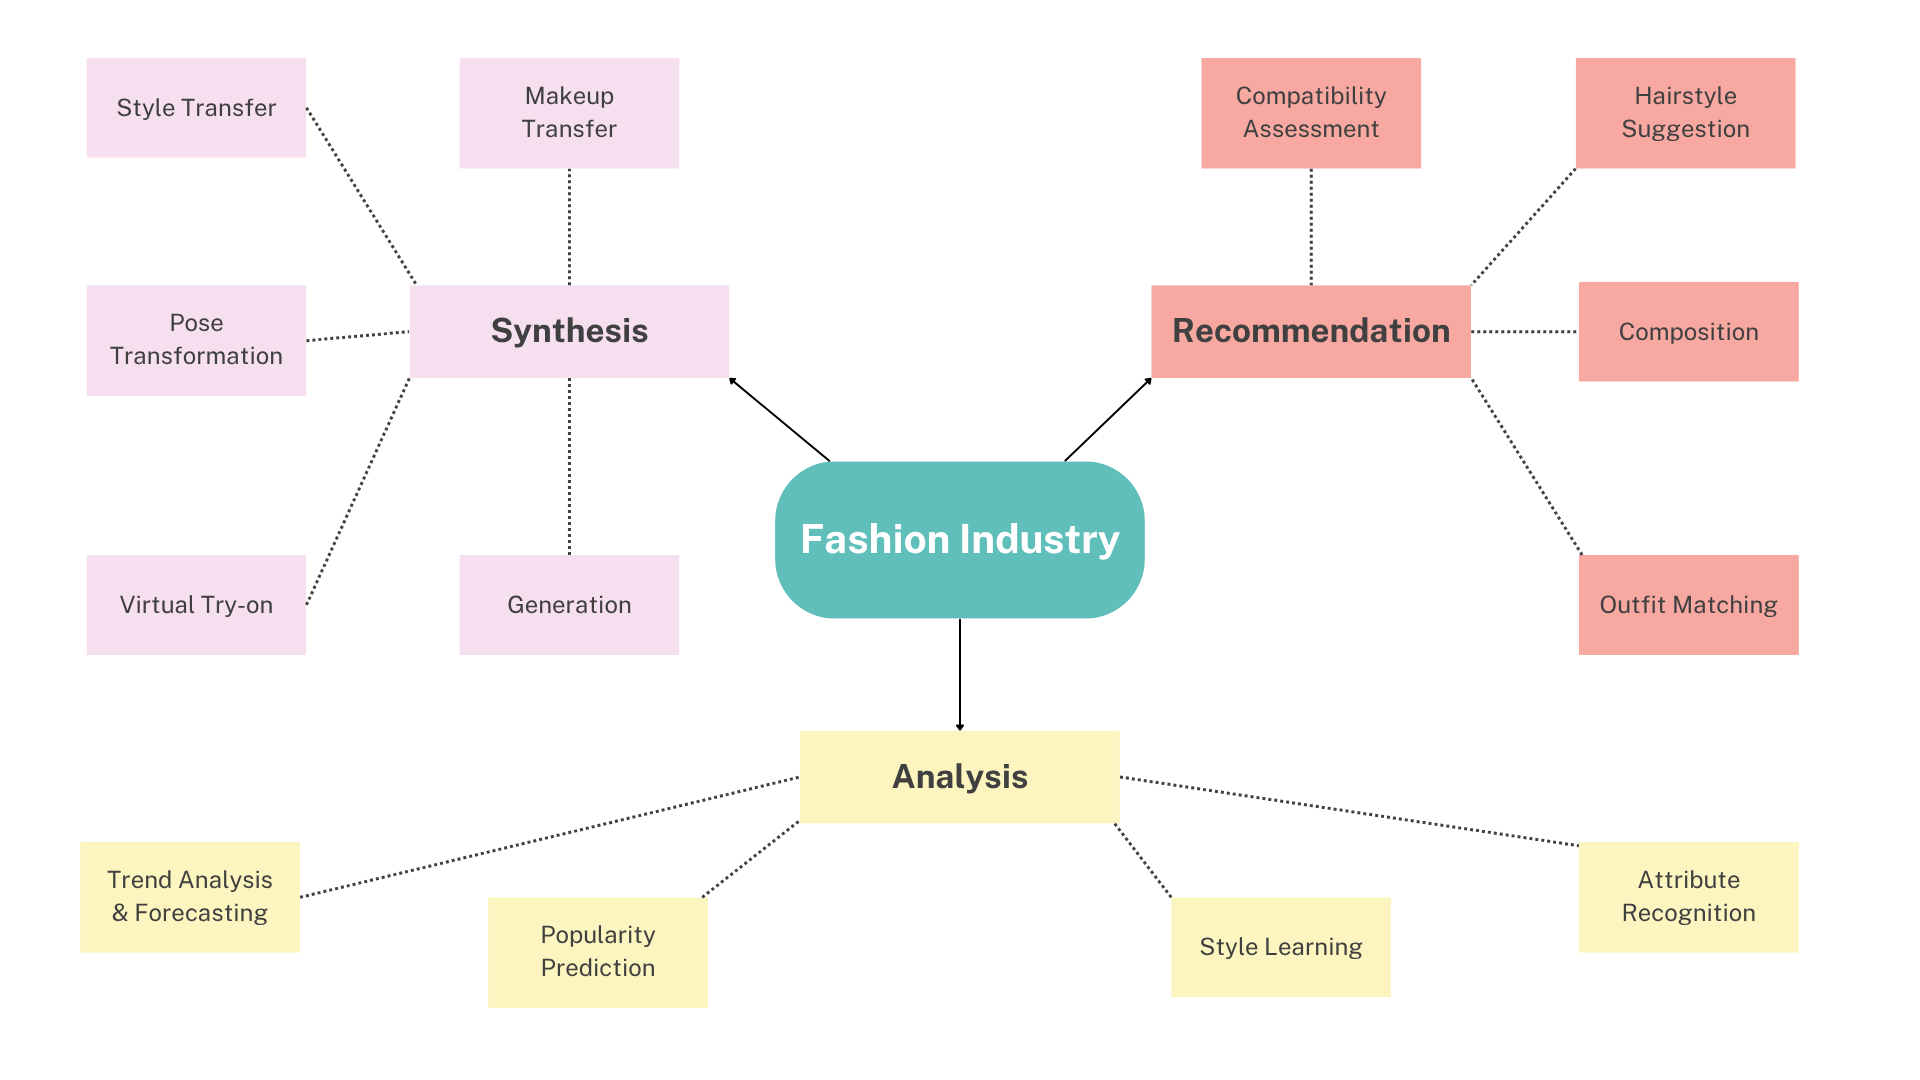
\includegraphics[width=\linewidth]{Abbildungen/fashion-areas.png}
  \caption{AI in Fashion (Mindmap)}
  \label{fig:fashion-areas}
\end{figure}

The goal of fashion recommendation is to automatically provide users with advice on what looks best on them and how to improve their style. This compatibility assessment is commonly associated with the task of outfit matching, where the overall collaboration between fashion items such as tops, bottoms, shoes, accessories is measured. \cite[cf.]{chen_survey_2023}

\section{Relevant Techniques in Outfit Matching and Compatibility Evaluation}

Outfit matching and compatibility evaluation combine principles from fashion theory, \acs{DL} and \acs{CV} to assess how well clothing items harmonize. This section explores key techniques, starting with foundational rules and progressing to computational models used in previous work.

\subsection{Techniques within Fashion Theory}

Compatibility evaluation among fashion items is typically modeled through fashion recommendation systems, which can broadly be divided into two categories: similar item recommendation and complementary recommendation. The former focuses on image retrieval techniques that suggest visually similar or identical fashion pieces. The latter aims to recommend items that complete or enhance a given outfit. \cite[cf.]{shirkhani_study_2023}

\vspace{0.5cm}

\textbf{Complementary Recommendation:}

\vspace{0.5cm}

This type of system includes three strategies. First, item recommendation predicts a single missing item based on a specific category. Second, outfit recommendation or outfit completion involves assembling a full outfit from scratch or adding items to an existing one. Third, capsule wardrobe generation seeks to propose a minimal yet versatile collection of items that can be mixed and matched into various outfits.

Complementary recommendation can further be distinguished based on context (e.g. product-based, scene-based, occasion-based) and evaluation scope (e.g. pair-wise, list-wise, set-wise).

\textbf{Context.}
Product-based methods assess the compatibility between items by analyzing their visual features, typically using product images. Scene-based approaches go a step further by incorporating contextual details such as the season, location or user-specific attributes. Finally, occasion-based recommendations tailor outfit suggestions to specific events, cultural settings or social contexts, ensuring relevance to the user's immediate needs.

\textbf{Evaluation.}
In terms of structure: pair-wise evaluation looks at two items at a time, list-wise methods consider a sequence of items and set-wise approaches treat the outfit as a whole, analyzing how well all the pieces work together.

\subsection{Techniques within \acs{ML}}

This section provides an overview of information that is foundational to this thesis. The methods are introduced both to establish a theoretical understanding and to contextualize their relevance within the review of related work and the implementation phase.

\vspace{0.5cm}

\textbf{\ac{CV}:}

\vspace{0.5cm}

In addressing the task of visually aware evaluation of the outfit composition, \acs{CV} is employed. \acs{CV} aims to create methods for computers to replicate the complexity of the human visual system by understanding digital images (e.g. photos, videos, other visual media) and extracting valuable information from them. \cite[cf.]{brownlee_deep_2019}

\vspace{0.5cm}

\textbf{\ac{DL}:}

\vspace{0.5cm}

In the context of this thesis, a \acs{DL} model, an algorithm that is modeled after the structure of the human brain, acts as a foundational element. These models consist of layers of interconnected neurons that process and transform input data. The weights of the connections between neurons in the network are adjusted over time to recognize patterns in data that are relevant to a specific task. Thereby, complex representations of data are automatically learned. \cite[cf.]{muller_introduction_2017}

\vspace{0.5cm}

\textbf{\ac{CNN}.}
Some popular \acs{DL} architectures include \acs{CNN}, which process images by applying small, learnable filters over pixel regions. These filters extract local features such as edges or textures. As the image passes through multiple convolutional layers, the network builds a hierarchical representation. The deeper layers of the network are capturing increasingly complex and abstract features that are useful for tasks like classification or detection. \cite[cf.]{oshea_introduction_2015}

To train a model, its parameters (weights and biases) are adjusted to reduce the loss, which measures the difference between predictions and true values. This is done using gradients, computed via backpropagation, which tells each layer how to update its parameters. In very deep networks, however, gradients can become extremely small as they are passed backward, causing earlier layers to learn very little. This is known as the vanishing gradient problem. Special architectures (e.g. \acs{ResNet}) can address this by helping gradients flow more effectively during training. \cite[cf.]{he_deep_2015} 

\vspace{0.5cm}

\textbf{\ac{ResNet}.}
One of the key \acs{CNN} models in fashion is \acs{ResNet}. Its key feature is the use of "skip/residual connections" across layers. These connections perform mappings that skip one or more layers and pass information directly to deeper layers. This network uses building blocks and lets each block learn a modification (residual) to its input, rather than the desired underlying function. Therefore, this model can handle very deep networks (with over 100 layers: e.g. ResNet-50, ResNet-101, ResNet-152), making it suitable for feature extraction from complex fashion datasets where high accuracy is required. \cite[cf.]{he_deep_2015}

\vspace{0.5cm}

\textbf{\ac{DeCNN}.}
\acs{DeCNN} inverts the operations of \acs{CNN} to reconstruct high-dimensional data (e.g. image segmentation, object detection, image synthesis). It leverages deconvolutional layers and unpooling, recovers spatial details lost during downsampling and learns hierarchical representations critical for both low-level (e.g. deblurring) and high-level (e.g. segmentation) tasks. \cite[cf.]{zeiler_deconvolutional_2010}

\vspace{0.5cm}

\textbf{\ac{RNN}.}
A \acs{RNN} is a class of neural networks designed to process sequential data, involving temporal or ordered data (e.g. language modeling or time-series prediction). It maintains a hidden state that captures information over time. However, the network often struggles with learning long-term dependencies due to issues such as vanishing gradients. \cite[cf.]{sherstinsky_fundamentals_2018}

\vspace{0.5cm}

\textbf{\ac{Bi-LSTM}.}
A \acs{Bi-LSTM} network is an advanced type of \acs{RNN} that addresses the aforementioned limitations. It processes sequential data in both forward and backward directions and combines their outputs to capture full context at every step. This architecture is especially powerful for tasks where understanding both past and future elements in a sequence is important. \cite[cf.]{huang_bidirectional_2015}

\vspace{0.5cm}

\textbf{\ac{RelNN}.}
A \acs{RelNN} is designed to tackle relational reasoning tasks by explicitly modeling how objects in a set relate to one another, rather than focusing solely on their individual properties. Given a set of object representations (e.g. features extracted from image regions using a \acs{CNN}, word embeddings from a sentence using a \ac{Bi-LSTM}) the model evaluates all possible pairs using a small neural network to capture their interactions. These pairwise relations are then aggregated and passed through another network to generate the final output. The architecture's ability to model structured interactions makes it applicable to domains involving object relationships such as evaluating visual harmony in outfit composition. \cite[cf.]{sung_learning_2018}

\vspace{0.5cm}

\textbf{Siamese Network.}
A Siamese (Twin) Network is a neural network architecture designed for similarity learning. Its goal is to determine how alike or different two inputs of the same modality (e.g. images) are. This network consists of a pair of neural networks that share their weights and aim at computing similarity functions. It learns to compare pairs of inputs by mapping them into a feature space where similar samples are close and dissimilar samples are far apart. This approach is powerful in fashion scenarios where the task involves verifying whether two samples belong to the same class (e.g. similar style despite differences in type or color). \cite[cf.]{koch_siamese_2015}

\vspace{0.5cm}

\textbf{\ac{VSE}.}
These models enable cross-modal tasks such as image-text retrieval, caption generation or visual question answering. Their goal is to align representations across different modalities (e.g. images and textual descriptions) in a shared vector space. \acs{CLIP} is a specific implementation of a \acs{VSE}-like model including important advancements. Fashion\acs{CLIP} is domain-adapted version of \acs{CLIP} which is fine-tuned and tailored specifically for fashion-related tasks. \cite[cf.]{faghri_vse_2018}

\vspace{0.5cm}

\textbf{\ac{MLP}.}
\acs{MLP} is a type of fully connected neural network composed of an input layer, one or more hidden layers with nonlinear activation functions and an output layer. While conceptually simple, \acsp{MLPs} are powerful function approximators and are commonly used in the final stages of many deep learning pipelines. In outfit recommendation or compatibility scoring tasks, \acsp{MLPs} are often employed to map high-level features that are extracted by earlier modules (e.g. \acs{CNN}, \acs{RNN}, \acs{RelNN}) into a final score representing the compatibility between items. \cite[cf.]{upgrad_overview_2023}

\vspace{0.5cm}

\textbf{Generative \ac{AI}.}
Generative \ac{AI} refers to a class of \ac{DL} models that can create new content (e.g. images, videos, music, text) by learning patterns from existing data. These models typically use self-supervised, unsupervised or weakly supervised techniques to capture the underlying structure of the data, rather than relying on fully labeled datasets. Depending on the approach, they may generate content unconditionally or be conditioned on input prompts or examples. A key feature of generative models is their ability to produce diverse and often realistic outputs. \cite[cf.]{sengar_generative_2024}

\vspace{0.5cm}

\textbf{\ac{GAN}.}
A \acs{GAN} is a framework where a generator and discriminator are trained in opposition. This results in a creation of highly realistic data. This process is widely used for image synthesis, data augmentation, text-to-image generation or style transfer. \cite[cf.]{goodfellow_generative_2014}

\section{Previous Work and Related Research}

Current section provides an overview of 10 papers that were choosen out of a total of 54. The selection process prioritized articles which are published within the last six years (from 2019 to 2025), written in English and are openly accessible. The search was conducted using specific terms such as "outfit compatibility", "fashion compatibility", "fashion recommendation", "deep learning", "aesthetic recommendation", "outfit generation" as well as a mix of these keywords. The most interesting articles based on their captions, abstracts and conclusions were subsequently downloaded and further investigated  in terms of their relevance to the use case. For all selected studies, their main goal and important technical elements are summarized below.

\textcolor{red}{remove hyperparameters later? check if all methods / techniques are explained earlier}

\vspace{0.5cm}

\textbf{Pairwise Approach:}

\vspace{0.5cm}

Wang et al. present a system that can predict whether a set of clothing items representing an outfit looks good and explain why it does (not). The developed network uses a \acs{CNN} (\acs{ResNet}-50) and \acs{GAP} to extract features from images of clothing items at different levels of abstraction. These features range from basic details such as color and texture (early layers) to more complex ones such as style and category (later layers). The extracted features are then used to compare each outfit item with every other outfit item in a pairwise comparison matrix. \acs{MLP} then produces a score that reflects the final overall compatibility score. Thus, both visual and textual information is integrated using \acs{VSE} which allows the model to learn a common representation between them. Gradient values generated by backpropagation are used to identify problematic pairs and to provide an explanation of why an outfit fails, pinpointing specific issues. As loss functions, the model employs binary cross-entropy and contrastive loss. The training is supervised. The model uses labeled data and learns with negative sampling. The prediction of compatibility is evaluated using metrics such as \acs{AUC} and \acs{FITB} accuracy. The key hyperparameters mentioned include: initial \acs{LR}: 0.01, decay factor: 0.2 every 10 epochs, \acs{CNN} depth: 4 layers, \acs{MLP} depth: 2 layers. \cite[cf.]{wang_outfit_2019}

\vspace{0.5cm}

\textbf{Relational Approach:}

\vspace{0.5cm}

Moosaei et al. tackle the challenge of creating a system that could 1) work with any number of clothing items 2) without needing a specific order and 3) without relying on traditional labels. First, \acs{RelNN} is used to treat each outfit as a "scene" and the items within it as "objects", thus learning how items relate to each other visually. After establishing the relationships, it combines them using \acs{MLP} to create a single score that indicates how well the outfit fits together. The authors also develop a more sophisticated version of the network that additionally incorporates textual information. DenseNet is used for visual feature extraction, one-hot encoding for textual features. The model uses cross-entropy loss. The training is supervised. The evaluation uses \acs{AUC} and \acs{FITB} accuracy. The key hyperparameters mentioned include: \acs{LR}: 0.001, batch size: 64, dropout rate: 0.35, epochs: 19, optimizer: Adam, \acs{MLP} depth: 4 layers (number of filters: 512, 512, 256, 256) + 3 layers (number of filters: 128, 128, 32). \cite[cf.]{moosaei_fashion_2020}

\vspace{0.5cm}

\textbf{Generative Approach and Template Generation:}

\vspace{0.5cm}

Liu et al. aim not only to measure compatibility but also to generate a "compatible template" that could help in understanding why certain pairings succeed or fail. The authors trained a \acs{GAN} on a massive dataset of clothing images paired with detailed textual descriptions to create a richer understanding of clothing compatibility. The architecture integrates downsampling, multi-modal fusion and upsampling. Convolutional layers are used for visual encoding, TextCNN for textual. The network learns to generate preliminary visual representations (templates) of what a compatible clothing item should look like based on a given one. \acs{AUC} and \acs{MRR} are used as metrics for evaluating the model. The \acs{LR} was set to 0.0002. \cite[cf.]{liu_mgcm_2020}

\vspace{0.5cm}

\textbf{Generative Approach:}

\vspace{0.5cm}

In another research, Moosaei et al. show a model used to generate compatible fashion items for an (incomplete) outfit. The developed model consists of two parts. The \acs{GAN} takes a partial outfit (images) along with a specified missing clothing item category (textual) as input and creates several potential outfit combinations. A compatibility network (\acs{CNN} + \acsp{MLPs} + \acs{RelNN}) checks if the generated item fits well with the rest of the outfit by identifying patterns in the relationships between items. It learns what makes different clothing items match each other based on their contextual relevance (relationships) and their visual aesthetics by incorporating the initial outfit input into its training. As a loss function, the model employs cross-entropy loss among others. Training is supervised for compatibility network and minimax game for \acs{GAN}. The prediction is evaluated using inception score, multi-scale structural similarity and compatibility score. \cite[cf.]{moosaei_outfitgan_2022}

\vspace{0.5cm}

\textbf{Graph-based Approach and Try-on Approach:}

\vspace{0.5cm}

Zheng et al. address item-by-item matching (collocation) and overall outfit appearance (try-on). Both of these perspectives are combined in a network to give a better evaluation of outfit compatibility. The developed model consists of two parts. \cite[cf.]{zheng_collocation_2021}

\begin{enumerate}
  \item The first part looks at each clothing item individually and checks how well they match with each other. This approach uses a disentangled \acs{GCN} and includes nodes (each representing clothing items), edges (showing the connections between items), condition masks (acting like filters that separate out different features of clothing items) and an attention mechanism (deciding which features are more crucial for determining if items match). Convolutional layers are used for visual features, \acs{ResNet}-like architecture for try-on images. 
  \item The second part imagines how the whole outfit would look when worn together and outputs the final try-on compatibility score. Thereby, the authors apply knowledge distillation and train a "teacher" network using available try-on images before transferring knowledge to a "student" network. This second network predicts how the outfit would look without the need for actual try-on images. Furthermore, item category information (such as top, bottom, etc.) is incorporated to understand the context of the outfit.
\end{enumerate}

In this paper, cross-entropy is chosen as a loss function, while the Kullback-Leibler divergence and L1 regularization are used as regularization terms. Instance normalization is applied. The training is semi-supervised with mutual learning strategy. The prediction of compatibility is evaluated using metrics such as \acs{AUC}, \acs{MRR}, \acs{HR} @1, @10, @100, @200. The key hyperparameters mentioned include: \acs{LR}: 0.0002, batch size: 32, optimizer: Adam, activation function: \acs{ReLU} (and Tanh), \acs{GCN} depth: one 1-strided convolutional layer and four 2-strided convolutional layers (number of filters: 32, 64, 128, 256, and 512, respectively), teacher network depth: same as \acs{GCN} for encoder + transform block composed of 6 residual blocks + decoder with four 2-strided deconvolutional layers and one 1-strided convolutional layer (number of filters: 32, 64, 128, 256, 512, 512, 512, 512, 512, 512, 512, 256, 128, 64, 32 and 3, respectively). \cite[cf.]{zheng_collocation_2021}

\vspace{0.5cm}

\textbf{Graph-based Approach:}

\vspace{0.5cm}

Work done by Guan et al. presents a system designed to automate the assessment of outfit compatibility while dealing with irregular attribute labels, information loss during disentanglement and combining different levels of information. The system tackles this through a three-stage methodology: \cite[cf.]{guan_partially_2022}

\begin{enumerate}
  \item It leverages a pre-trained model (\acs{ResNet}-18) to extract visual features from each clothing item. \acsp{MLPs} are applied to break these features down into attributes (partially supervised disentangled learning). Despite the fact that the generated attribute labels are irregular, this partially supervised approach is used to guide the attribute-level learning.
  \item To prevent losing information during breakdown, the authors introduce two strategies: orthogonal residual embedding layers (layers that reintroduce missing information) and visual representation reconstruction (a \acs{DeCNN} that reconstructs the original image from fragmented attributes).
  \item The system builds a graph where nodes represent fashion items and edges represent compatibility relationships (e.g. "matches", "does not match", "requires modification"). Hierarchical \acs{GCN} is implemented to model the relationships between clothing items, considering both attribute-level and item-level compatibility. The final compatibility score is derived from the combination of both results.
\end{enumerate}

In this paper, cross-entropy is chosen as a loss function, while orthogonal regularization is used as a regularization term. The evaluation uses \acs{AUC} and \acs{FITB} accuracy. The key hyperparameters mentioned include: \acs{LR}: 0.0001, batch size: 32, optimizer: Adam, \acs{GCN} depth: 1 layer, \acs{DeCNN} depth: 5 transposed layers (output dimension: 256), \acsp{MLPs} depth: 2 layers (for each label with output dimension: 64), activation functions: LeakyReLU, \acs{ReLU}, Tanh. \cite[cf.]{guan_partially_2022}

\vspace{0.5cm}

\textbf{Colors and Textures:}

\vspace{0.5cm}

Kim et al. implement a model that can learn from unlabeled data using \acs{SCL} and suggest items that complement each other based on shared color palettes and textures. On the one hand, the model learns to predict the distribution of colors present in images and to recognize color patterns. On the other hand, it learns to identify and recognize different textures (such as stripes, polka dots, etc.). Additionally, in order to filter out irrelevant information (e.g. shape), the model focuses on smaller, independent image patches and learns to identify the types of colors and textures present within these patches. The architecture consists of \acs{CNN} (\acs{ResNet}-50) and separate projection heads for sub-tasks. Contrastive loss (for shapeless local patch discrimination, texture discrimination) is chosen as a loss function, while the Kullback-Leibler divergence (for RGB histograms) and L1 regularization are used as regularization terms. The prediction is evaluated using \acs{AUC}, \acs{FITB} accuracy, recall@K. The key hyperparameters mentioned include: \acs{LR}: 0.00005, optimizer: Adam, activation function: \acs{ReLU}, epochs: 150, heads depth: two fully connected layers. \cite[cf.]{kim_self-supervised_2020}

\vspace{0.5cm}

\textbf{Styles and Textures:}

\vspace{0.5cm}

Dong et al. present a system that can automatically generate matching clothing items while considering style and texture using \acs{SSL}. This is done without requiring pairs of outfits that already match, instead mapping an input image of a clothing item to a complementary image. The network utilizes three main parts: \cite[cf.]{dong_towards_2025}

\begin{enumerate}
  \item First component (discriminator with \acs{ResNet} backbon and \acsp{MLPs}) helps the system understand the style and texture representations of the input clothing. Later on it ensures that the synthesized clothing is compatible with the input clothing in terms of style and texture.
  \item The second component (dual discriminator) ensures that the generated images are realistic and visually coherent. One discriminator is designed to favor real images (positive samples) and assigns high scores to latent codes produced by the encoding network, while the other discriminator favors generated images (negative samples) and assigns high scores to latent codes produced by the mapping network. Conversely, the first discriminator assigns low scores to latent codes from the mapping network, and the second assigns low scores to latent codes from the encoding network.
  \item Build upon \acs{GAN} inversion, the last component (generator) uses a pre-trained model (StyleGAN) to understand the basic structure of clothing. It then applies style and texture information to generate a matching image, guided by the DST and dual discriminator losses.
\end{enumerate}

\vspace{0.5cm}

\textbf{Body Shape:}

\vspace{0.5cm}

Pang et al. designed a model that generates outfit recommendations that prioritize both visual compatibility and body shape suitability. This is achieved through a layered architecture that incorporates: \cite[cf.]{pang_learning_2024}

\begin{enumerate}
  \item Seven body shape representations with 3D body models, measurements and front-view images captured from multiple angles for each body shape. These are used to train the model to understand the overall silhouette using \acs{SMPL} and \acs{ResNet}.
  \item This part extracts visual features from images that show how an outfit looks when worn (available or generated with M-VTON) using \acs{ResNet}. It also generates textual descriptions of clothing attributes using \acs{GloVe}. Both are then represented as vector representations.
  \item The final part of the model combines body shape representation and outfit representation into a single, unified representation. Cross-modal attention is used to identify correlations between body shape and outfit attributes, focus on the most relevant features when making recommendations and provide explanations for why an outfit is recommended.
\end{enumerate}

Thereby, binary cross-entropy loss is chosen as a loss function. The evaluating metrics include \acs{AUC}, mean average precision, average per-class precision, recall, F1 score, average overall precision. The key hyperparameters mentioned are: \acs{LR}: 0.1, batch size: 10, optimizer: SDG, activation function: \acs{ReLU}, weight decay: 0.0005, momentum: 0.9. \cite[cf.]{pang_learning_2024}

\vspace{0.5cm}

\textbf{Occasion:}

\vspace{0.5cm}

In their work, Vo et al. create a system that can tell if different clothing items are compatible for specific occasions beyond simple style matching. The authors designed a framework with three main parts: \cite[cf.]{vo_efficient_2023}

\begin{enumerate}
  \item \acs{Bi-LSTM} analyzes the entire outfit as a sequence (like words in a sentence) and learns how different clothing items relate to each other.
  \item \acs{ResNet}-50 extracts visual features from clothing images and \acs{VSE} connects them to textual descriptions (one-hot encoded) to understand visual style and matching.
  \item The last part focuses specifically on recognizing if an outfit is suitable for a particular occasion. It uses an auxiliary classifier with global average pooling, fully connected layers and softmax to classify outfits based on occasions.
\end{enumerate}

The system is evaluated using metrics such as \acs{AUC} and \acs{FITB} accuracy. As a loss function, it employs triplet loss and cross-entropy loss among others. The key hyperparameters mentioned include: batch size: 10, initial \acs{LR}: 0.2, then changed by a factor of 2 for every two epochs. \cite[cf.]{vo_efficient_2023}

\chapter{Proposed Solutions}

This chapter presents an overview of potential solution approaches relevant to the task of visual outfit evaluation within the field of \acs{CV}. The main goal of the desired solution is to extract features from images, evaluate matching and compute overall compatibility score. 

\section{Overarching Framework}

Based on an in-depth review of related literature, the specific use case and the available resources, a general direction for the solution has been defined: a \acs{GAN}-inspired architecture is most suitable for addressing the challenges of this task.

The generator-like component acts as an outfit creator (template-guided or as a random combiner of clothing items). The discriminator-like component evaluates the quality of these outfits and assigns an aesthetic rating (1-10). The outfit creation process is then iteratively refined based on feedback (e.g. from the scoring model, from the user).

This approach simulates the functionality of a \acs{GAN} without actually implementing a full network and avoiding the complexity of training it. It leverages existing pre-trained models and techniques in a creative way, making it both feasible and resource-efficient. However, without a true generator-discriminator loop, the carefull design of the interaction of generator-like and discriminator-like components is am important task.

\section{Individual Components}

While the overarching framework is clear, the implementation of individual components within this architecture can vary significantly. Therefore, this section explores a range of alternative methods for each key module, analyzing their respective strengths, limitations and applicability.

The different modules in the choosen strategy are illustrated in Figure \ref{fig:workflow-modules} and described bellow.

\begin{figure}[h]
  \centering
  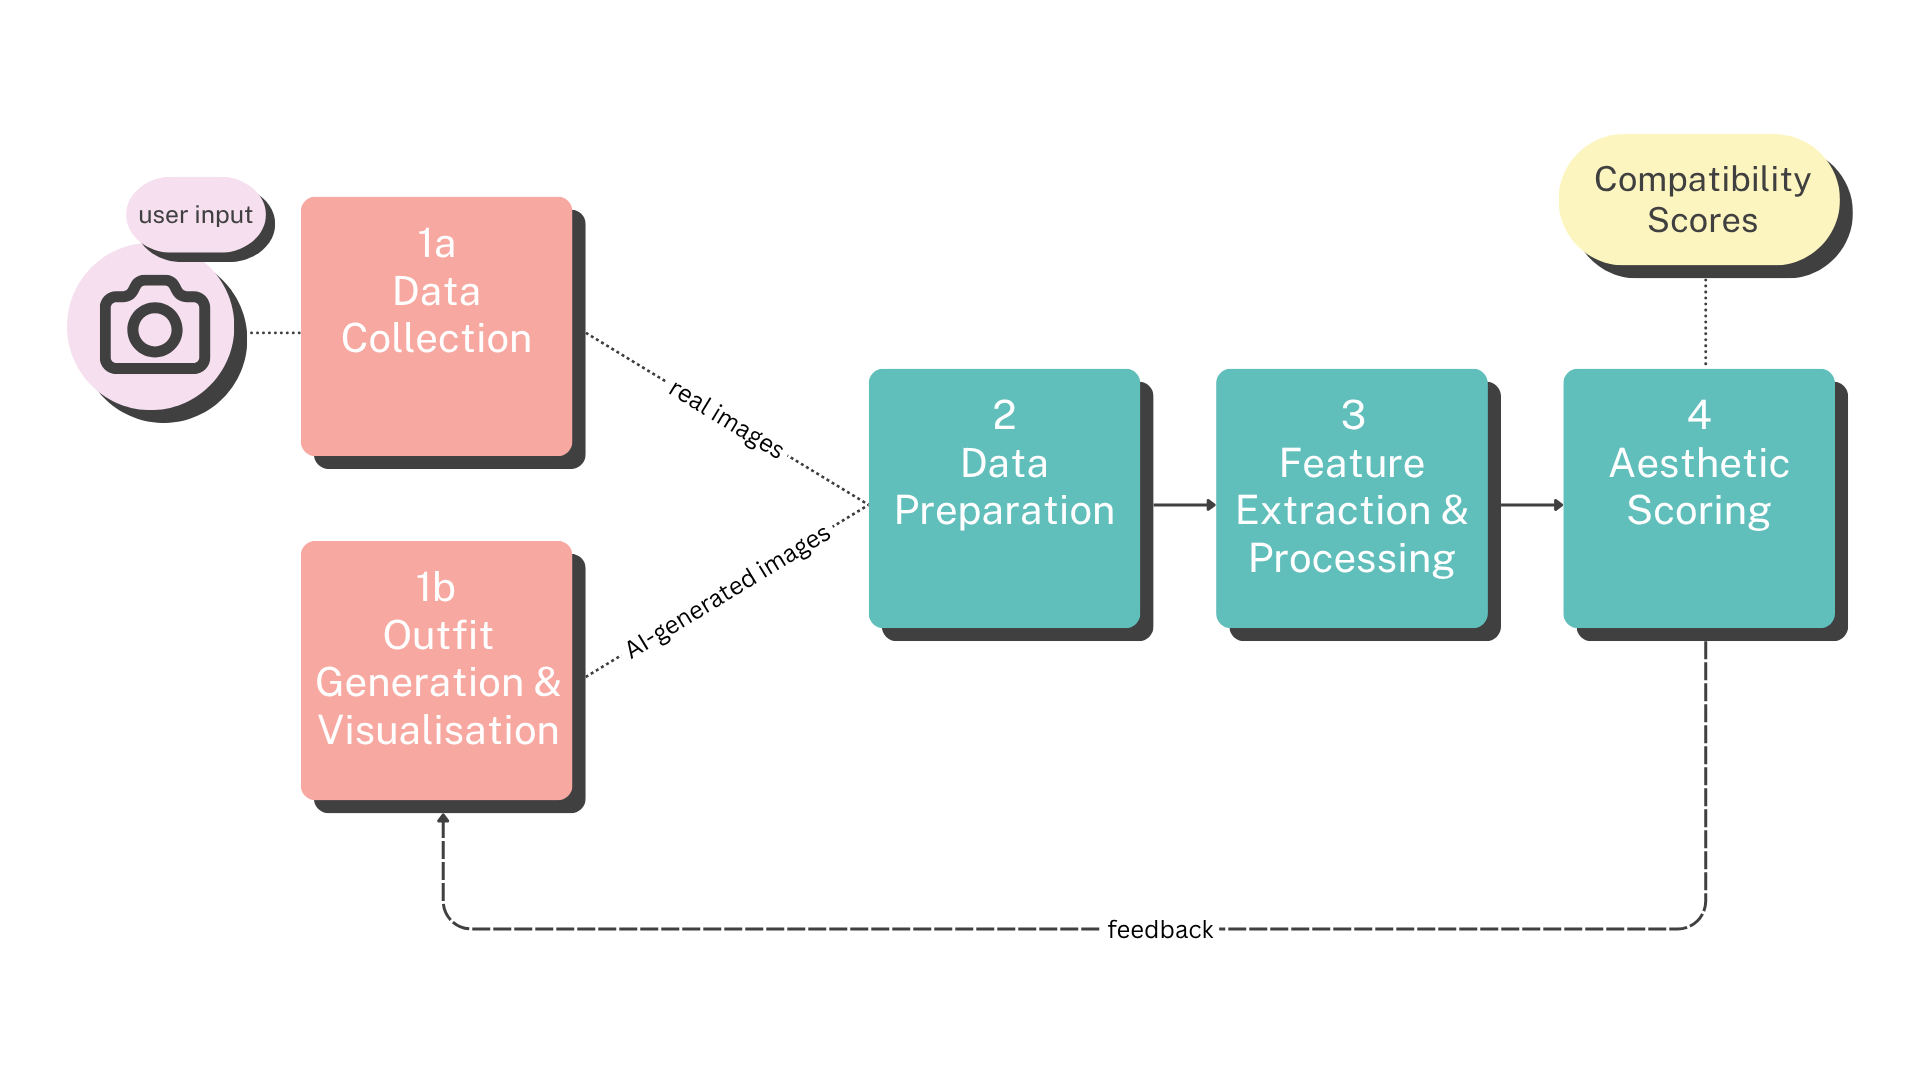
\includegraphics[width=\linewidth]{Abbildungen/workflow-modules.png}
  \caption{\acs{GAN}-Inspired System and its Modules (Workflow)}
  \label{fig:workflow-modules}
\end{figure}

\subsection{Data Collection Module (1a)}

The data collection strategy must align with the chosen method to learn data representations. In this work, two relevant approaches are considered: \acs{NC-SSL} and \acs{SCL}. These methods influence how data should be organized.

\vspace{0.5cm}

\textbf{Positive Pairs (\ac{NC-SSL}).}
This approach that relies exclusively on positive sample pairs and data augmentations. These are well-balanced and stylish outfits, typically sourced from fashion experts or curated user sets.

\vspace{0.5cm}

\textbf{Positive and Negative Pairs (\ac{SCL}).}
This learning strategy uses both positive and negative pairs. While the positive examples remain the same as in the previous approach, negative samples consist of visually unappealing outfits (e.g. those with clashing colors, disproportionate silhouettes, excessive layering).

\vspace{0.5cm}

\textbf{Comparative Analysis:}

\vspace{0.5cm}

Both, positive and negative outfit data samples can be sourced from platforms like Pinterest and Google or from public datasets such as DeepFashion, Polyvore and FashionGen. While there are some positive outfit examples available, identifying truly representative positive and negative samples remains difficult. This is because the quality of an outfit is often subjective. This means, that what looks good to one person might not appeal to another. As a result, both positive and negative samples require human evaluation, ideally with personalization in mind. Randomizing outfit pieces can help generate negative examples, but the results are often unrealistic or too obviously mismatched. Moreover, many bad outfits are only subtly off, making them hard to label without contextual knowledge. Collecting a well-balanced dataset, therefore, demands time and careful curation.

\vspace{0.5cm}

\textbf{Selected Approach incl. Justification:}

\vspace{0.5cm}

Due to the challenges in obtaining reliable contrastive data the decision is made to begin with a non-contrastive training strategy, using only known good outfits. This allows the model to first learn what makes an outfit aesthetically and semantically coherent. Once the training is finished and the model can reliably score outfits using the discriminator-like component, the generator-like component creates outfit combinations and recieves scores. Out of these newly generated outfits, only high- or low-scoring examples are selected for further training. This self-bootstrapping strategy gradually improves the model without relying on manually labeled negative samples.

Current approach is also suitable for a possible future phase, where each user is able to provide a personalized outfit history containing both liked and disliked looks. This allows the model to fine-tune its understanding of style preferences on an individual level, using real user behavior as training input for personalized outfit scoring.

Furthermore, in later stages, additional data can be gathered through user-uploaded outfits, styled looks from partner brands, second-hand shops, or stylists, as well as previously \acs{AI}-generated combinations as discribed in the module 1b.

\subsection{Outfit Generation and Visualisation Module (1b)}

A few approaches to generate and display fashion outfits are being explored:

\vspace{0.5cm}

\textbf{Random Outfit Generation.}
As a baseline, outfits can be randomly sampled by selecting items across predefined categories (e.g. top, bottom, shoes, accessories). While these combinations are unstructured, they allow evaluation of the model's ability to detect outfit quality without prior structure.

\vspace{0.5cm}

\textbf{Rule-Based and Template-Guided Generation.}
This approach imposes structural constraints on outfit creation, provides interpretability and guides the generation of coherent outfits. Fashion heuristics and predefined templates are used. For instance, the \href{https://medium.com/@snc5440/the-8-point-rule-of-fashion-31180d957925}{8-Point Rule of Fashion} offers a quantitative framework where each item contributes a defined number of "style points", promoting visual balance and coherence. These constraints can be applied during generation or as a post-processing filter to refine candidate outfits. Additionally, users can personalize the rule system, enabling flexible alignment with subjective fashion preferences.

\vspace{0.5cm}

\textbf{Outfit Visualisation.}
One way to display an \acs{AI}-generated outfit is by using \acs{IDM-VTON} to place segmented clothing items on a person. This virtual try-on network ensures that generated outfits look realistic and contextually appropriate. However, it may not handle all body shapes or poses perfectly or lead to a computational overhead if used extensively.

\vspace{0.5cm}

\textbf{Comparative Analysis:}

\vspace{0.5cm}

\textcolor{red}{text missing}

\vspace{0.5cm}

\textbf{Selected Approach incl. Justification:}

\vspace{0.5cm}

Rules are used as a starting point but allow the model to deviate based on learned patterns. \textcolor{red}{text missing}

\subsection{Data Preparation Module (2)}

Both modules 1a and 1b feed raw images incl. optional metadata (style, weather, event, gender, tags) into an aesthetic scoring model. The data needs to be processed accordingly in this module.

\vspace{0.5cm}

\textbf{Image Data.}
To prepare images several preprocessing steps are involved. The process begins with object detection or clothing item recognition, which identifies garments using models such as YOLOv8, Detectron2, Grounding DINO or fine-tuned EfficientNet. Following detection, segmentation is applied to isolate clothing items from the background using techniques such as \acs{SAM}, Mask R-CNN or SegFormer. Next valuable step is pose estimation and pose normalization, which helps to understand how items are worn and ensures consistent alignment (e.g. mapping a person to a standard pose). Applying this step would make the comparison between outfits more fair and easier (all images in the same pose = easier to judge fit and compatibility). In order to do pose estimation, tools like OpenPose, MediaPipe or HRNet can be used. Once the relevant clothing regions are identified, cropping and background removal is used to focus solely on the garments. This is done by leveraging segmentation results to crop the items and removing the background using models such as U2Net, RemBG or \acs{SAM}. To ensure consistency in the dataset, images are then resized to a typical resolution (e.g. 224x224 or 512x512) and pixel values are normalized (e.g. to a [0, 1] range). Optionally, data augmentation is utilized to improve generalization.

\vspace{0.5cm}

\textbf{Textual Data.}
When raw image data is accompanied by textual metadata such as descriptions, tags, captions or user comments, it is important to preprocess this information to ensure consistency and usefulness. The first step involves cleaning the text, which includes removing special characters, emojis, irrelevant hashtags and links, as well as normalizing whitespace and converting the text to lowercase. Next, the pipeline includes a text filtering stage to remove uninformative or noisy content. Once the text is cleaned and filtered, it undergoes tokenization, which depends on the model in use.

\vspace{0.5cm}

\textbf{Comparative Analysis:}

\vspace{0.5cm}

\textcolor{red}{text missing}

\vspace{0.5cm}

\textbf{Selected Approach incl. Justification:}

\vspace{0.5cm}

\textcolor{red}{text missing}

\subsection{Feature Extraction and Processing Module (3)}

Ensuring that the system learns meaningful relationships between clothing items and aesthetic ratings requires careful feature engineering. This module captures basic visual attributes such as color and texture. It also learns additional, more complex features, such as color harmony, texture matching, balance, contrast and composition. These features align with human intuition about fashion aesthetics. They add depth to the model's understanding of what makes an outfit "good" and are crucial for evaluating outfit quality.

\vspace{0.5cm}

\textbf{Image Data: Fine Tuning.}
This approach takes a single pre-trained model and fine-tunes it so that it is adapted to new data patterns. The model can then perform the desired tasks on its own. A pre-trained ResNet can be taken and continued to be trained on own data to extract complex features from outfit images (e.g. outfit quality, style labels, embeddings).

\vspace{0.5cm}

\textbf{Textual Data.}
After tokenization, the pipeline proceeds with semantic embedding extraction, transforming the processed text into vector representations. Fashion\acs{CLIP} is preferred for fashion-specific contexts, but alternatives such as \acs{CLIP}, BERT, SBERT, Sentence-T5 or \acs{GloVe} can be used. Optionally, metadata fusion can be applied by converting the attributes into descriptive prompts (e.g. “A red wool sweater with a relaxed fit”) or encoding them as key-value pairs for structured input formats.

\vspace{0.5cm}

\textbf{Ensemble Modeling.}
This is a strategy of using multiple pre-trained networks in order to extract diverse features. It combines outputs from multiple feature extractors, focusing on the strengths of different models, and improves robustness and generalization. However, it may increase computational overhead and requires careful fusion of features from different models.

The output includes cleaned images, segmentation masks and structured metadata.


, which evaluates the generated outfits using learned visual-semantic embeddings (e.g., from FashionCLIP) and learned similarity metrics.



Based on that, the module also refines the features to better represent the outfit's aesthetic qualities. To process the extracted features, an \acs{MLP} can be implemented.

\vspace{0.5cm}

\textbf{Comparative Analysis:}

\vspace{0.5cm}

\textcolor{red}{text missing}

\vspace{0.5cm}

\textbf{Selected Approach incl. Justification:}

\vspace{0.5cm}

\textcolor{red}{text missing}

\subsection{Aesthetic Scoring Module (4)}

This module uses the processed features to predict an aesthetic score. There are two options:

\begin{enumerate}
   \item It can be a simple linear layer or another \acs{MLP} layer to output a score between 0 and 1, which can be scaled to a percentage.
   \item Siamese network can be used to learn similarity-based scoring. This approach allows for meaningful comparisons between outfits, clustering similar outfits and separating dissimilar ones. The quality of the embedding space depends on the diversity of the dataset.
\end{enumerate}

\vspace{0.5cm}

\textbf{Comparative Analysis:}

\vspace{0.5cm}

\textcolor{red}{text missing}

\vspace{0.5cm}

\textbf{Selected Approach incl. Justification:}

\vspace{0.5cm}

\textcolor{red}{text missing}

---------------------------
Both of the explained ideas can be combined. First, multiple specialized models are pre-trained (e.g. a CLIP for semantics, a pose-sensitive model, a garment classifier). Later, an ensemble fusion model is fine-tuned 
on your task (e.g. outfit scoring, quality ranking, similarity).
This way, your Feature Extraction Module is not just plug-and-play — it's a powerful fashion intelligence layer.
Suggestion:
- Start with simpler features like color harmony and balance, which can be computed using computer vision techniques.
- Use pre-trained models or libraries (e.g., ColorThief) to analyze color palettes.
- Gradually incorporate more complex features as the system evolves.
- Start with a small ensemble of two or three models (e.g., one for global features and one for local details).
- Use late fusion (e.g., concatenating outputs) or attention mechanisms to combine features effectively.

Future Research Directions (For Thesis): Investigate the use of machine learning to *dynamically* adjust compatibility rules based on the current outfit's characteristics. Develop a system that allows users to provide more detailed style preferences and integrate these preferences into the generation process. Extend the system to generate outfits that synthesize elements from multiple existing style guidelines, creating unique and novel combinations. - While the output is visually appealing, integration notes suggest a further refinement of the compatibility criteria, potentially incorporating factors like color palettes, silhouette considerations, and formality level.  The system performs well with common garment types - shirts, pants, dresses - but struggles with more complex combinations.

- Use Siamese networks or triplet loss to create an embedding space where similar outfits are closer together.
- Incorporate additional features (e.g., color harmony, balance) into the scoring process.


Key Takeaways
1. Focus on Feasibility: Avoid computationally expensive tasks (e.g., training a GAN) and leverage pre-trained models wherever possible.
2. Prioritize Key Features: Begin with essential features like color harmony, balance, and similarity-based scoring before adding complexity.
3. Iterative Development: Develop the system incrementally, starting with a simple prototype and refining it based on feedback.
4. User-Centric Design: Ensure the final product is engaging and useful for users, with opportunities for personalization and interaction.

proposed a translation-based neural fashion compatibility model which contained three parts: (1) first mapped each item into a latent space via two CNN for visual and textual modality, (2) encoded the category complementary relations into the latent space, and (3) minimized a margin-based ranking criterion to optimize both item embeddings and relation vectors jointly.

Score compatible with me
Score compatible with every other piece I am wearing or could buy

compatibility clothing with me and clothing with eachother

items of clothes (segmented)
whole outfit
person segmented

relations (scores)


splitting it up? possibility
explainable AI -> highlight the least compatible item


The final section provides a justification for the selected combination of techniques, aligning each choice with the project goals and practical constraints.
\chapter{Implementation}

The following sections detail the system architecture, technical stack and specific implementation choices.

\section{System Architecture and Technical Stack}

\section{Implementation of Selected Approach}

The implementation follows a step-by-step procedure. Initially, fundamental features such as color harmony, balance and similarity-based scoring are prioritized before introducing more complex elements. The system is developed incrementally, starting with a basic prototype and refining it progressively based on experimental results. This iterative process is essential for building a robust and effective solution. Ultimately, the final product aims to be engaging and user-friendly, offering opportunities for personalization and interaction.

Start with simpler features like color harmony and balance, which can be computed using computer vision techniques.
- Use pre-trained models or libraries (e.g., ColorThief) to analyze color palettes.
- Gradually incorporate more complex features as the system evolves.
- Start with a small ensemble of two or three models (e.g., one for global features and one for local details).
- Use late fusion (e.g., concatenating outputs) or attention mechanisms to combine features effectively.
- Use Siamese networks or triplet loss to create an embedding space where similar outfits are closer together.
- Incorporate additional features (e.g., color harmony, balance) into the scoring process.

\section{Data Collection and Preprocessing}


1. Data Preparation: Ensure your dataset includes diverse outfits with corresponding aesthetic scores.
2. Normalization: Normalize input images to ensure consistency.
3. Hyperparameter Tuning: Experiment with different learning rates, batch sizes, and number of epochs.
4. Validation Strategy: Use a validation set to monitor performance and prevent overfitting.

Data Collection: The first step is to gather labeled data, which typically consists of input features and their corresponding target labels. This data should be representative of the problem you want to solve.
Data curation: The process of cleaning and organizing the collected data to ensure its quality and reliability. This step involves removing any outliers or inconsistencies, handling missing values, and transforming the data into a suitable format for training the model.
Data Splitting: The collected data is usually divided into two subsets: the training dataset and the test data. Train the model with the training dataset, while the test data is reserved for evaluating its performance.

segmentation masks and structured metadata

\textbf{Textual Data.}

After tokenization, the pipeline proceeds with semantic embedding extraction, transforming the processed text into vector representations. Fashion\acs{CLIP} is preferred for fashion-specific contexts, but alternatives such as \acs{CLIP}, BERT, SBERT, Sentence-T5 or \acs{GloVe} can be used. Optionally, metadata fusion can be applied by converting the attributes into descriptive prompts (e.g. “A red wool sweater with a relaxed fit”) or encoding them as key-value pairs for structured input formats.

\section{AI Model Development and Training}

Model Selection: Depending on the problem at hand, you choose an appropriate supervised learning algorithm. For example, if you're working on a classification task, you might opt for algorithms like logistic regression, support vector machines, or decision trees.
Training the Model: This step involves feeding the training data into the chosen algorithm, allowing the model to learn the patterns and relationships in the data. The training iteratively adjusts its parameters to minimize prediction errors with its learning techniques.
Model Evaluation: After training, you evaluate the model's performance using the test set. Standard evaluation metrics include accuracy, precision, recall, and F1-score.
Fine-tuning: If the model's performance is unsatisfactory, you may need to fine-tune its hyperparameters or consider more advanced algorithms. This step is crucial for improving the model's accuracy.
Deployment: Once you're satisfied with the model's performance, you can deploy it to make predictions on new, unseen data in real-world applications.

Fine-Tuning Techniques

\href{https://viso.ai/deep-learning/pose-estimation-ultimate-overview/}{Human Pose Estimation reference}

SAM
category-guided attention mechanisms


\href{https://encord.com/blog/mastering-supervised-learning-a-comprehensive-guide/}{Supervised learning reference}
\href{https://blog.dataiku.com/outfit-recommendation-system}{Building an AI-Powered Outfit Recommendation System With Dataiku}
\href{https://nisargdoshi.medium.com/smart-fashion-recommendation-using-resnet50-b21d47cc91b1}{Smart Fashion Recommendation using ResNet50}
\chapter{Evaluation and Testing}
\section{Experimental Setup and Test Scenarios}

Fashion Compatibility.
Fill in the Black (FITB).
Fashion Retrieval.


\section{Performance Metrics and Evaluation Criteria}
\section{Results and Observations}

\clearpage
\phantomsection
\addcontentsline{toc}{chapter}{References}
\printbibliography


\chapter*{Statement of Affirmation}
\addcontentsline{toc}{chapter}{Statement of Affirmation}
I hereby declare that all parts of this thesis were exclusively prepared by me, without using resources other than those stated above. The thoughts taken directly or indirectly from external sources are appropriately annotated. This thesis or parts of it were not previously submitted to any other academic institution and have not yet been published.

\vspace{3cm}
\noindent
Dornbirn, July 2025 \hfill Viktoriia Simakova

\end{document}